\section{Introduction}
Advanced robotic technology has opened up the possibility of integrating highly autonomous robots into shared workspaces with human teams. These \textit{collaborative} robots are envisioned to increase productivity of human labor, allow greater flexibility in production, and improve ergonomics of manual tasks \cite{peshkin1999cobots, tan2009human}. However, this capability raises the question of how to best allocate work to maximize team efficiency and the experience of human team members working with robotic teammates.
       
While prior work on task allocation for teams of humans and robots, i.e., \textit{human-robot teaming}, has explored methods for allocating work for minimizing makespan, or task completion time, and ergonomic impact \cite{shah2011improved, gombolay2014decision, tsarouchi2017ijcim}, other factors exist that can affect worker experience with collaborating with robots, overall job satisfaction, and eventually the widespread adoption of collaborative robots. One such factor is \textit{task homogeneity}---whether we assign tasks such that a robot and its human collaborator work on different, specialized set of tasks (i.e., non-homogenous) or such that they work on the same set of non-specialized tasks (i.e., homogeneous). When task homogeneity is high, human and robot workers share workspace, tools, and supplies, which may increase the need for coordination. Another factor that may affect worker experience in task allocation is \textit{task interdependence} \cite{kiggundu1983task}---whether tasks are allocated such that human and robot workers depend on each other for completing the task or work in parallel without any dependency. Higher task interdependence requires increased coordination between human and robot teammates. 

\begin{figure}[t!]
	\caption{In this paper, we investigate how task and worker characteristics affect participants' perceptions of a robotic collaborator and their work, using a simulated manufacturing workcell in which the human-robot team work together under different task allocations.}\vspace{4pt}
	\label{fig:teaser}
	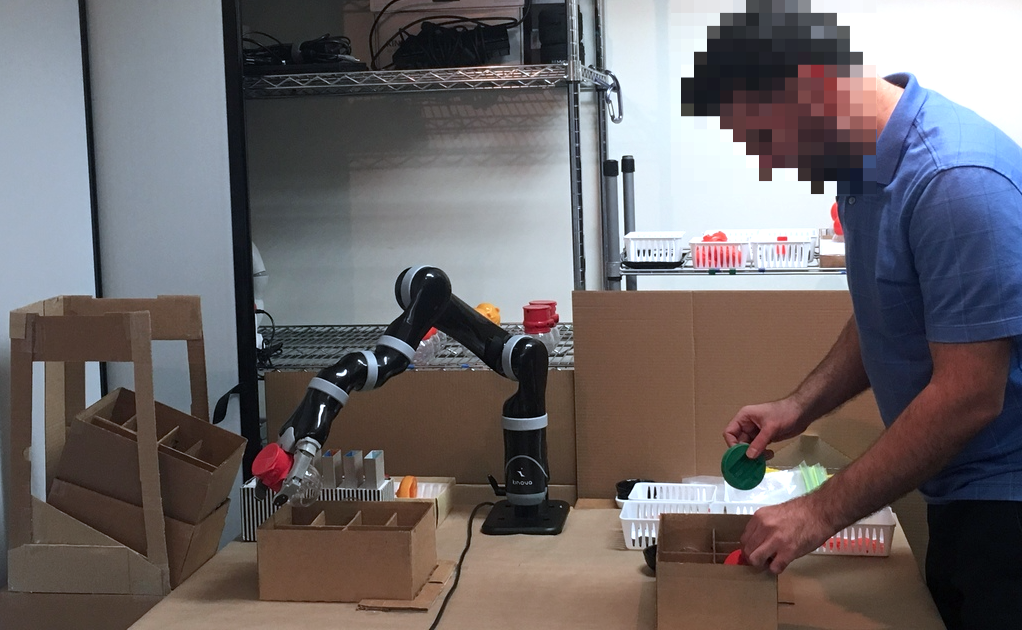
\includegraphics[width=\columnwidth]{figures/teaser.png}
\end{figure} 

While prior work on human-only teams has explored how job specialization and interdependence can affect workers' self-efficacy, job satisfaction, and team outcomes \cite{miller1973job,kuijer1999job,hsieh2004reassessment}, how these factors translate to human-robot teams remains unknown. Furthermore, worker characteristics may add to this complexity. For example, human-robot interaction literature highlight stark differences in how men and women interact with robots  \cite{schermerhorn2008robot}, suggesting that \textit{worker sex} may be one of the factors that shape worker experience with collaborative robots.
       
In this paper, we study how task interdependence, homogeneity, and worker characteristics, particularly sex, affect psychological outcomes of human-robot teaming for human workers, such as perceptions of robotic teammates, perceptions of collaboration, and perceptions of work using a simulated manufacturing workcell created in our laboratory (Figure \ref{fig:teaser}). The results of this study can guide us in more effective task allocation for human-robot teams.
